% Practice Test 14 — Virginia Edition
% Questions: 30 (21 MC + 9 SA)
% Generated by scripts/generate_practice_tests.py

\begin{practiceQuestion}{1-4-q02}{mc}
\begin{questionText}
The table shows a proportional relationship. Which equation represents it?

\begin{center}
\begin{tabular}{|c|c|}
\hline $x$ & $y$ \\ \hline $4$ & $10$ \\ $6$ & $15$ \\ $10$ & $25$ \\ \hline
\end{tabular}
\end{center}
\end{questionText}
\choiceA{$y = 4x$}
\choiceB{$y = 2.5x$}
\choiceC{$y = x + 6$}
\choiceD{$y = 10x$}
\correctAnswer{B}
\explanation{$k = \frac{10}{4} = 2.5$. The equation is $y = 2.5x$. Check: $2.5 \times 6 = 15$ and $2.5 \times 10 = 25$ \checkmark.}
\end{practiceQuestion}

\begin{practiceQuestion}{2-1-q22}{sa}
\begin{questionText}
A jar has $250$ candies. If $44\%$ are chocolate, how many chocolate candies are there?
\end{questionText}
\correctAnswer{$110$}
\explanation{$44\% = 0.44$. Multiply: $0.44 \times 250 = 110$ chocolate candies.}
\end{practiceQuestion}

\begin{practiceQuestion}{2-2-q08}{mc}
\begin{questionText}
$15$ is what percent of $125$?
\end{questionText}
\choiceA{$10\%$}
\choiceB{$12\%$}
\choiceC{$15\%$}
\choiceD{$18\%$}
\correctAnswer{B}
\explanation{$\frac{15}{125} = \frac{p}{100}$. Cross-multiply: $125p = 1500$. Divide: $p = 12\%$.}
\end{practiceQuestion}

\begin{practiceQuestion}{2-3-q29}{gsa}
\begin{questionText}
The bar graph shows a store's T-shirt inventory at the start and end of the week. What is the percent decrease?

\begin{center}
\begin{tikzpicture}[scale=0.55]
  \draw[thick,->] (0,0) -- (0,6.5) node[above]{\small T-shirts};
  \draw[thick,->] (0,0) -- (5.5,0);
  % Bars
  \fill[funBlue!60] (0.5,0) rectangle (2,5);
  \fill[funOrange!60] (2.5,0) rectangle (4,3);
  % Labels
  \node[below,font=\small] at (1.25,0) {Start};
  \node[below,font=\small] at (3.25,0) {End};
  \foreach \y/\lab in {1/20,2/40,3/60,4/80,5/100} {
    \draw (-0.1,\y) -- (0.1,\y) node[left,font=\small,xshift=-2pt] {\lab};
  }
  \node[above,font=\small] at (1.25,5) {$100$};
  \node[above,font=\small] at (3.25,3) {$60$};
\end{tikzpicture}
\end{center}
\end{questionText}
\correctAnswer{$40\%$}
\explanation{Change: $100 - 60 = 40$. Percent decrease: $40 \div 100 = 0.40 = 40\%$.}
\end{practiceQuestion}

\begin{practiceQuestion}{2-7-q29}{gsa}
\begin{questionText}
The table shows the results of a science experiment. Calculate the percent error for Trial 3 (round to the nearest tenth).

\begin{center}
\begin{tabular}{|l|c|c|c|}
\hline
 & \textbf{Predicted (g)} & \textbf{Actual (g)} & \textbf{Percent Error} \\
\hline
Trial 1 & $50$ & $48$ & $4.2\%$ \\
\hline
Trial 2 & $50$ & $55$ & $9.1\%$ \\
\hline
Trial 3 & $50$ & $44$ & ? \\
\hline
\end{tabular}
\end{center}
\end{questionText}
\correctAnswer{$\approx 13.6\%$}
\explanation{$\frac{|50 - 44|}{44} \times 100 = \frac{6}{44} \times 100 \approx 13.6\%$.}
\end{practiceQuestion}

\begin{practiceQuestion}{3-2-q20}{sa}
\begin{questionText}
What is $(-4) + (-4) + (-4)$?
\end{questionText}
\correctAnswer{$-12$}
\explanation{Three negatives with same sign: $4 + 4 + 4 = 12$. Keep the negative: $-12$.}
\end{practiceQuestion}

\begin{practiceQuestion}{3-3-q22}{sa}
\begin{questionText}
A bird is flying at $12$ meters above the ground. A fish is swimming at $-5$ meters (below sea level). What is the distance between them?
\end{questionText}
\correctAnswer{$17$ meters}
\explanation{$|12 - (-5)| = |12 + 5| = |17| = 17$ meters.}
\end{practiceQuestion}

\begin{practiceQuestion}{3-4-q24}{sa}
\begin{questionText}
What is $3.25 + (-5.5) + 1.75$?
\end{questionText}
\correctAnswer{$-0.5$}
\explanation{$3.25 + 1.75 = 5.0$. Then $5.0 + (-5.5) = -0.5$.}
\end{practiceQuestion}

\begin{practiceQuestion}{4-3-q18}{mc}
\begin{questionText}
Which shows the correct expansion of $-3(2x - 4y + 1)$?
\end{questionText}
\choiceA{$-6x + 12y - 3$}
\choiceB{$-6x - 12y - 3$}
\choiceC{$-6x + 12y + 3$}
\choiceD{$-6x - 12y + 1$}
\correctAnswer{A}
\explanation{$-3 \times 2x = -6x$, $-3 \times (-4y) = +12y$, and $-3 \times 1 = -3$. Result: $-6x + 12y - 3$.}
\end{practiceQuestion}

\begin{practiceQuestion}{4-4-q17}{mc}
\begin{questionText}
Factor $9x + 12x + 15x$ using the GCF.
\end{questionText}
\choiceA{$3x(3 + 4 + 5)$}
\choiceB{$3(3x + 4x + 5x)$}
\choiceC{$x(9 + 12 + 15)$}
\choiceD{$9x(1 + 12 + 15)$}
\correctAnswer{A}
\explanation{GCF is $3x$. Divide each: $9x \div 3x = 3$, $12x \div 3x = 4$, $15x \div 3x = 5$. Result: $3x(3 + 4 + 5)$. This simplifies to $3x(12) = 36x$.}
\end{practiceQuestion}

\begin{practiceQuestion}{5-4-q07}{mc}
\begin{questionText}
Solve $\dfrac{3n}{4} + 6 = 15$.
\end{questionText}
\choiceA{$n = 28$}
\choiceB{$n = 12$}
\choiceC{$n = 7$}
\choiceD{$n = 36$}
\correctAnswer{B}
\explanation{Subtract $6$: $\frac{3n}{4} = 9$. Multiply by $4$: $3n = 36$. Divide by $3$: $n = 12$. Check: $\frac{3(12)}{4} + 6 = 9 + 6 = 15$ \checkmark.}
\end{practiceQuestion}

\begin{practiceQuestion}{5-5-q06}{mc}
\begin{questionText}
Solve $-4x > 20$.
\end{questionText}
\choiceA{$x > -5$}
\choiceB{$x < -5$}
\choiceC{$x > 5$}
\choiceD{$x < 5$}
\correctAnswer{B}
\explanation{Divide by $-4$ and flip the sign: $x < -5$.}
\end{practiceQuestion}

\begin{practiceQuestion}{5-6-q28}{gmc}
\begin{questionText}
Look at the two number lines below. Which statement is true?

\textbf{Line 1:}
\begin{center}
\begin{tikzpicture}[scale=0.55]
  \draw[thick,->] (-6,0) -- (6,0);
  \foreach \x in {-5,...,5} \draw (\x,0.12) -- (\x,-0.12) node[below,font=\small] {$\x$};
  \draw[thick,funBlue,->] (-3,0) -- (6,0);
  \fill[funBlue] (-3,0) circle (4pt);
\end{tikzpicture}
\end{center}

\textbf{Line 2:}
\begin{center}
\begin{tikzpicture}[scale=0.55]
  \draw[thick,->] (-6,0) -- (6,0);
  \foreach \x in {-5,...,5} \draw (\x,0.12) -- (\x,-0.12) node[below,font=\small] {$\x$};
  \draw[thick,funOrange,->] (-3,0) -- (6,0);
  \draw[thick,funOrange,fill=white] (-3,0) circle (4pt);
\end{tikzpicture}
\end{center}
\end{questionText}
\choiceA{Both graphs include $-3$ as a solution}
\choiceB{Line 1 shows $x \geq -3$ and Line 2 shows $x > -3$}
\choiceC{Line 1 shows $x > -3$ and Line 2 shows $x \geq -3$}
\choiceD{Both graphs represent the same inequality}
\correctAnswer{B}
\explanation{Line 1 has a closed circle (includes $-3$): $x \geq -3$. Line 2 has an open circle (excludes $-3$): $x > -3$.}
\end{practiceQuestion}

\begin{practiceQuestion}{6-1-q04}{mc}
\begin{questionText}
On a map, $2$ cm represents $50$ km. What is the scale factor?
\end{questionText}
\choiceA{$2$ km per cm}
\choiceB{$25$ km per cm}
\choiceC{$50$ km per cm}
\choiceD{$100$ km per cm}
\correctAnswer{B}
\explanation{Find the unit rate: $50 \div 2 = 25$ km per cm.}
\end{practiceQuestion}

\begin{practiceQuestion}{6-2-q01}{mc}
\begin{questionText}
A map uses the scale $1$ cm $= 50$ km. You redraw it at $1$ cm $= 25$ km. A road that is $6$ cm on the original map becomes how long on the new map?
\end{questionText}
\choiceA{$3$ cm}
\choiceB{$6$ cm}
\choiceC{$12$ cm}
\choiceD{$150$ cm}
\correctAnswer{C}
\explanation{Scale ratio: $\frac{50}{25} = 2$. New length: $6 \times 2 = 12$ cm. The new scale is more detailed, so the drawing gets bigger.}
\end{practiceQuestion}

\begin{practiceQuestion}{6-5-q03}{mc}
\begin{questionText}
You slice a cone with a horizontal cut parallel to its base. What shape is the cross-section?
\end{questionText}
\choiceA{A circle smaller than the base}
\choiceB{A circle the same size as the base}
\choiceC{A triangle}
\choiceD{A rectangle}
\correctAnswer{A}
\explanation{A horizontal cut through a cone parallel to the base produces a circle smaller than the base. The higher you cut, the smaller the circle.}
\end{practiceQuestion}

\begin{practiceQuestion}{6-6-q17}{mc}
\begin{questionText}
An angle is $12°$ less than its complement. What is the angle?
\end{questionText}
\choiceA{$39°$}
\choiceB{$42°$}
\choiceC{$48°$}
\choiceD{$51°$}
\correctAnswer{A}
\explanation{Let the angle be $x$ and its complement be $x + 12$. Sum: $x + (x + 12) = 90$. Combine: $2x + 12 = 90$. Solve: $2x = 78$, $x = 39°$.}
\end{practiceQuestion}

\begin{practiceQuestion}{6-7-q26}{gmc}
\begin{questionText}
The graph shows triangle $ABC$ and its image $A'B'C'$. What transformation was performed?

\begin{center}
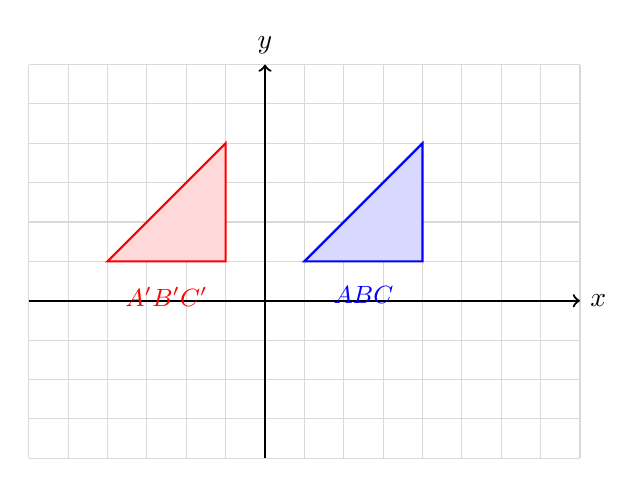
\begin{tikzpicture}[scale=0.5]
  \draw[step=1,gray!30,thin] (-6,-4) grid (8,6);
  \draw[thick,->] (-6,0) -- (8,0) node[right]{$x$};
  \draw[thick,->] (0,-4) -- (0,6) node[above]{$y$};
  % Original
  \draw[thick,blue,fill=blue!15] (1,1) -- (4,1) -- (4,4) -- cycle;
  \node[blue,below] at (2.5,0.6) {\small $ABC$};
  % Image
  \draw[thick,red,fill=red!15] (-4,1) -- (-1,1) -- (-1,4) -- cycle;
  \node[red,below] at (-2.5,0.6) {\small $A'B'C'$};
\end{tikzpicture}
\end{center}
\end{questionText}
\choiceA{Translation left $5$}
\choiceB{Reflection over the $y$-axis}
\choiceC{Rotation $90°$ clockwise}
\choiceD{Reflection over the $x$-axis}
\correctAnswer{B}
\explanation{Each point's $x$-coordinate is negated while $y$ stays the same: $(1,1) \to (-1,1)$, $(4,1) \to (-4,1)$, $(4,4) \to (-4,4)$. This is a reflection over the $y$-axis.}
\end{practiceQuestion}

\begin{practiceQuestion}{6-8-q12}{mc}
\begin{questionText}
Which method can you use to find a missing side in similar figures?
\end{questionText}
\choiceA{Add the same number to each known side}
\choiceB{Set up a proportion with corresponding sides}
\choiceC{Subtract the scale factor from the known side}
\choiceD{Multiply all sides by the number of vertices}
\correctAnswer{B}
\explanation{In similar figures, corresponding sides are proportional. Set up $\frac{\text{side}_1}{\text{corresponding side}_1} = \frac{\text{side}_2}{\text{corresponding side}_2}$ and cross-multiply.}
\end{practiceQuestion}

\begin{practiceQuestion}{7-4-q20}{sa}
\begin{questionText}
A figure is a rectangle $15$ m by $8$ m with a rectangular hole $5$ m by $3$ m cut out. What is the area of the remaining figure?
\end{questionText}
\correctAnswer{$105$ m$^2$}
\explanation{Outer: $15 \times 8 = 120$ m$^2$. Hole: $5 \times 3 = 15$ m$^2$. Remaining: $120 - 15 = 105$ m$^2$.}
\end{practiceQuestion}

\begin{practiceQuestion}{7-5-q06}{mc}
\begin{questionText}
A gift box is $8$ cm by $5$ cm by $3$ cm. How much wrapping paper is needed to cover the entire box?
\end{questionText}
\choiceA{$79$ cm$^2$}
\choiceB{$120$ cm$^2$}
\choiceC{$158$ cm$^2$}
\choiceD{$316$ cm$^2$}
\correctAnswer{C}
\explanation{$SA = 2(8 \times 5) + 2(8 \times 3) + 2(5 \times 3) = 80 + 48 + 30 = 158$ cm$^2$.}
\end{practiceQuestion}

\begin{practiceQuestion}{7-6-q22}{sa}
\begin{questionText}
A rectangular aquarium is $80$ cm long, $40$ cm wide, and $50$ cm tall. What is its volume in cubic centimeters?
\end{questionText}
\correctAnswer{$160{,}000$ cm$^3$}
\explanation{$V = 80 \times 40 \times 50 = 160{,}000$ cm$^3$.}
\end{practiceQuestion}

\begin{practiceQuestion}{7-7-q28}{gmc}
\begin{questionText}
Two cylinders are shown. Cylinder A has radius $2$ cm and height $9$ cm. Cylinder B has radius $3$ cm and height $4$ cm. Which cylinder has the greater volume? Use $\pi \approx 3.14$.

\begin{center}
\begin{tikzpicture}[scale=0.3]
  % Cylinder A
  \draw[thick,funBlue] (-7,0) ellipse (2 and 0.7);
  \draw[thick,funBlue] (-9,0) -- (-9,9);
  \draw[thick,funBlue] (-5,0) -- (-5,9);
  \draw[thick,funBlue] (-7,9) ellipse (2 and 0.7);
  \node[below] at (-7,-1.5) {Cylinder A};
  \node[left,funRed] at (-9.5,4.5) {$h = 9$};
  \node[above,funRed] at (-7,10) {$r = 2$};
  % Cylinder B
  \draw[thick,funRed] (7,0) ellipse (3 and 0.7);
  \draw[thick,funRed] (4,0) -- (4,4);
  \draw[thick,funRed] (10,0) -- (10,4);
  \draw[thick,funRed] (7,4) ellipse (3 and 0.7);
  \node[below] at (7,-1.5) {Cylinder B};
  \node[right,funRed] at (10.5,2) {$h = 4$};
  \node[above,funRed] at (7,5) {$r = 3$};
\end{tikzpicture}
\end{center}
\end{questionText}
\choiceA{Cylinder A}
\choiceB{Cylinder B}
\choiceC{They have the same volume}
\choiceD{Not enough information}
\correctAnswer{C}
\explanation{A: $V = 3.14 \times 4 \times 9 = 113.04$ cm$^3$. B: $V = 3.14 \times 9 \times 4 = 113.04$ cm$^3$. They have the same volume.}
\end{practiceQuestion}

\begin{practiceQuestion}{8-1-q06}{mc}
\begin{questionText}
A city wants to survey residents about a new park. Which method would produce the least biased sample?
\end{questionText}
\choiceA{Survey people at the existing park}
\choiceB{Put the survey in the newspaper and wait for responses}
\choiceC{Randomly select addresses from the city directory}
\choiceD{Survey people at the city council meeting}
\correctAnswer{C}
\explanation{Randomly selecting addresses gives all residents an equal chance, reducing bias.}
\end{practiceQuestion}

\begin{practiceQuestion}{8-3-q25}{sa}
\begin{questionText}
Two groups have means of $50$ and $54$, and both have MAD $= 8$. Express the difference in means as a multiple of MAD. Is the difference meaningful?
\end{questionText}
\correctAnswer{$0.5$ MADs; no, the difference is not meaningful}
\explanation{$\frac{54-50}{8} = 0.5$ MADs. Since $0.5 < 2$, the difference is small relative to the variability and not considered meaningful.}
\end{practiceQuestion}

\begin{practiceQuestion}{8-4-q27}{gmc}
\begin{questionText}
The box plots show quiz scores (out of $20$) for two classes.

\begin{center}
\begin{tikzpicture}[scale=0.35]
  \draw[thick,->] (4,0) -- (21,0);
  \foreach \x in {5,6,...,20} {
    \draw (\x,0.3) -- (\x,-0.3);
    \node[below,font=\tiny] at (\x,-0.3) {$\x$};
  }
  % Class M: min=8, Q1=12, med=15, Q3=17, max=20
  \draw[thick] (8,3) -- (20,3);
  \draw[thick,fill=funBlue!30] (12,2) rectangle (17,4);
  \draw[very thick,funBlue] (15,2) -- (15,4);
  \draw[thick] (8,2) -- (8,4);
  \draw[thick] (20,2) -- (20,4);
  \node[right,font=\small] at (20.5,3) {Class M};
  % Class N: min=10, Q1=13, med=16, Q3=18, max=19
  \draw[thick] (10,7) -- (19,7);
  \draw[thick,fill=funGreen!30] (13,6) rectangle (18,8);
  \draw[very thick,funGreen] (16,6) -- (16,8);
  \draw[thick] (10,6) -- (10,8);
  \draw[thick] (19,6) -- (19,8);
  \node[right,font=\small] at (19.5,7) {Class N};
\end{tikzpicture}
\end{center}

What is the IQR for each class?
\end{questionText}
\choiceA{Class M: $5$, Class N: $5$}
\choiceB{Class M: $12$, Class N: $9$}
\choiceC{Class M: $5$, Class N: $9$}
\choiceD{Class M: $12$, Class N: $5$}
\correctAnswer{A}
\explanation{Class M: $Q_3 - Q_1 = 17 - 12 = 5$. Class N: $18 - 13 = 5$. Both have IQR $= 5$.}
\end{practiceQuestion}

\begin{practiceQuestion}{8-5-q09}{mc}
\begin{questionText}
What is the median of this data set?

\begin{center}
\begin{tabular}{r|l}
\textbf{Stem} & \textbf{Leaf} \\
\hline
$6$ & $0\;\;3\;\;5$ \\
$7$ & $1\;\;4\;\;7\;\;8$ \\
$8$ & $2\;\;6$
\end{tabular}
\end{center}
\end{questionText}
\choiceA{$71$}
\choiceB{$74$}
\choiceC{$77$}
\choiceD{$75.5$}
\correctAnswer{B}
\explanation{Data: $60, 63, 65, 71, 74, 77, 78, 82, 86$. There are $9$ values; the $5$th (middle) is $74$.}
\end{practiceQuestion}

\begin{practiceQuestion}{9-3-q16}{mc}
\begin{questionText}
A weather station recorded rain on $36$ out of $120$ days last spring. Based on this data, what is the experimental probability of rain on any spring day?
\end{questionText}
\choiceA{$0.36$}
\choiceB{$0.30$}
\choiceC{$0.25$}
\choiceD{$0.03$}
\correctAnswer{B}
\explanation{$P = \frac{36}{120} = 0.30$.}
\end{practiceQuestion}

\begin{practiceQuestion}{9-6-q11}{mc}
\begin{questionText}
Two dice are rolled. What is the probability that the sum is even?
\end{questionText}
\choiceA{$\frac{1}{4}$}
\choiceB{$\frac{1}{3}$}
\choiceC{$\frac{1}{2}$}
\choiceD{$\frac{2}{3}$}
\correctAnswer{C}
\explanation{Even sums occur when both dice are even or both are odd. Both even: $3 \times 3 = 9$. Both odd: $3 \times 3 = 9$. Total: $18$ out of $36$. $P = \frac{18}{36} = \frac{1}{2}$.}
\end{practiceQuestion}

\begin{practiceQuestion}{9-7-q03}{mc}
\begin{questionText}
To simulate an event with a $\frac{1}{6}$ probability, which tool would be most appropriate?
\end{questionText}
\choiceA{A coin}
\choiceB{A standard die}
\choiceC{A spinner with $4$ sections}
\choiceD{A bag with $2$ marbles}
\correctAnswer{B}
\explanation{A standard die has $6$ equally likely outcomes, each with probability $\frac{1}{6}$.}
\end{practiceQuestion}
